\documentclass[aspectratio=169]{beamer}
\setbeamertemplate{navigation symbols}{}
\usepackage{color,amsmath,comment, subfigure}
\usepackage{booktabs}
\usepackage{url}

%\setbeameroption{show notes}

%%%%%%%%%%%%%%%%%%%%%%%%%%
\title[]{Class 8: Spread of disease in networks}
\author[]{Matthew J. Salganik}
\institute[]{Sociology 204: Social Networks, Spring 2021\\Princeton University}
\date[]{
2/3:  Networks and sexually transmitted diseases
\vfill 

\begin{flushleft}
\vspace{0.6in}

\includegraphics[width=0.1\textwidth]{figures/cc.png}
\end{flushleft}

}

\note{
TODO: Move candy bowl to the end of this class possibly. Helps set the stage for next class and has them do it before they see the readings
TODO: Try to find movie of chains of affection
}

\begin{document}
%%%%%%%%%%%%%%%%%%%%%%%%%%%
\frame{\titlepage}
%%%%%%%%%%%%%%%%%%%%%%%%%%%
\begin{comment}
\begin{frame}

SWBAT:
\begin{enumerate}
\end{enumerate}

\end{frame}
\end{comment}
%%%%%%%%%%%%%%%%%%%%%%%%%%%%%
\begin{frame}

\begin{center}
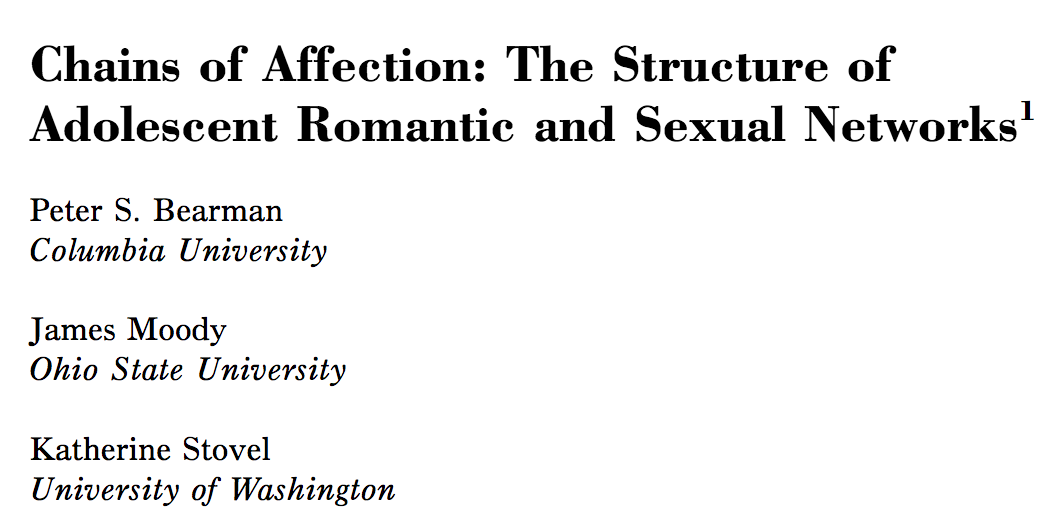
\includegraphics[width = 0.95\textwidth]{figures/bearman_chains_2004_title}
\end{center}

\end{frame}
%%%%%%%%%%%%%%%%%%%%%%%%%%%
\begin{frame}

\begin{center}
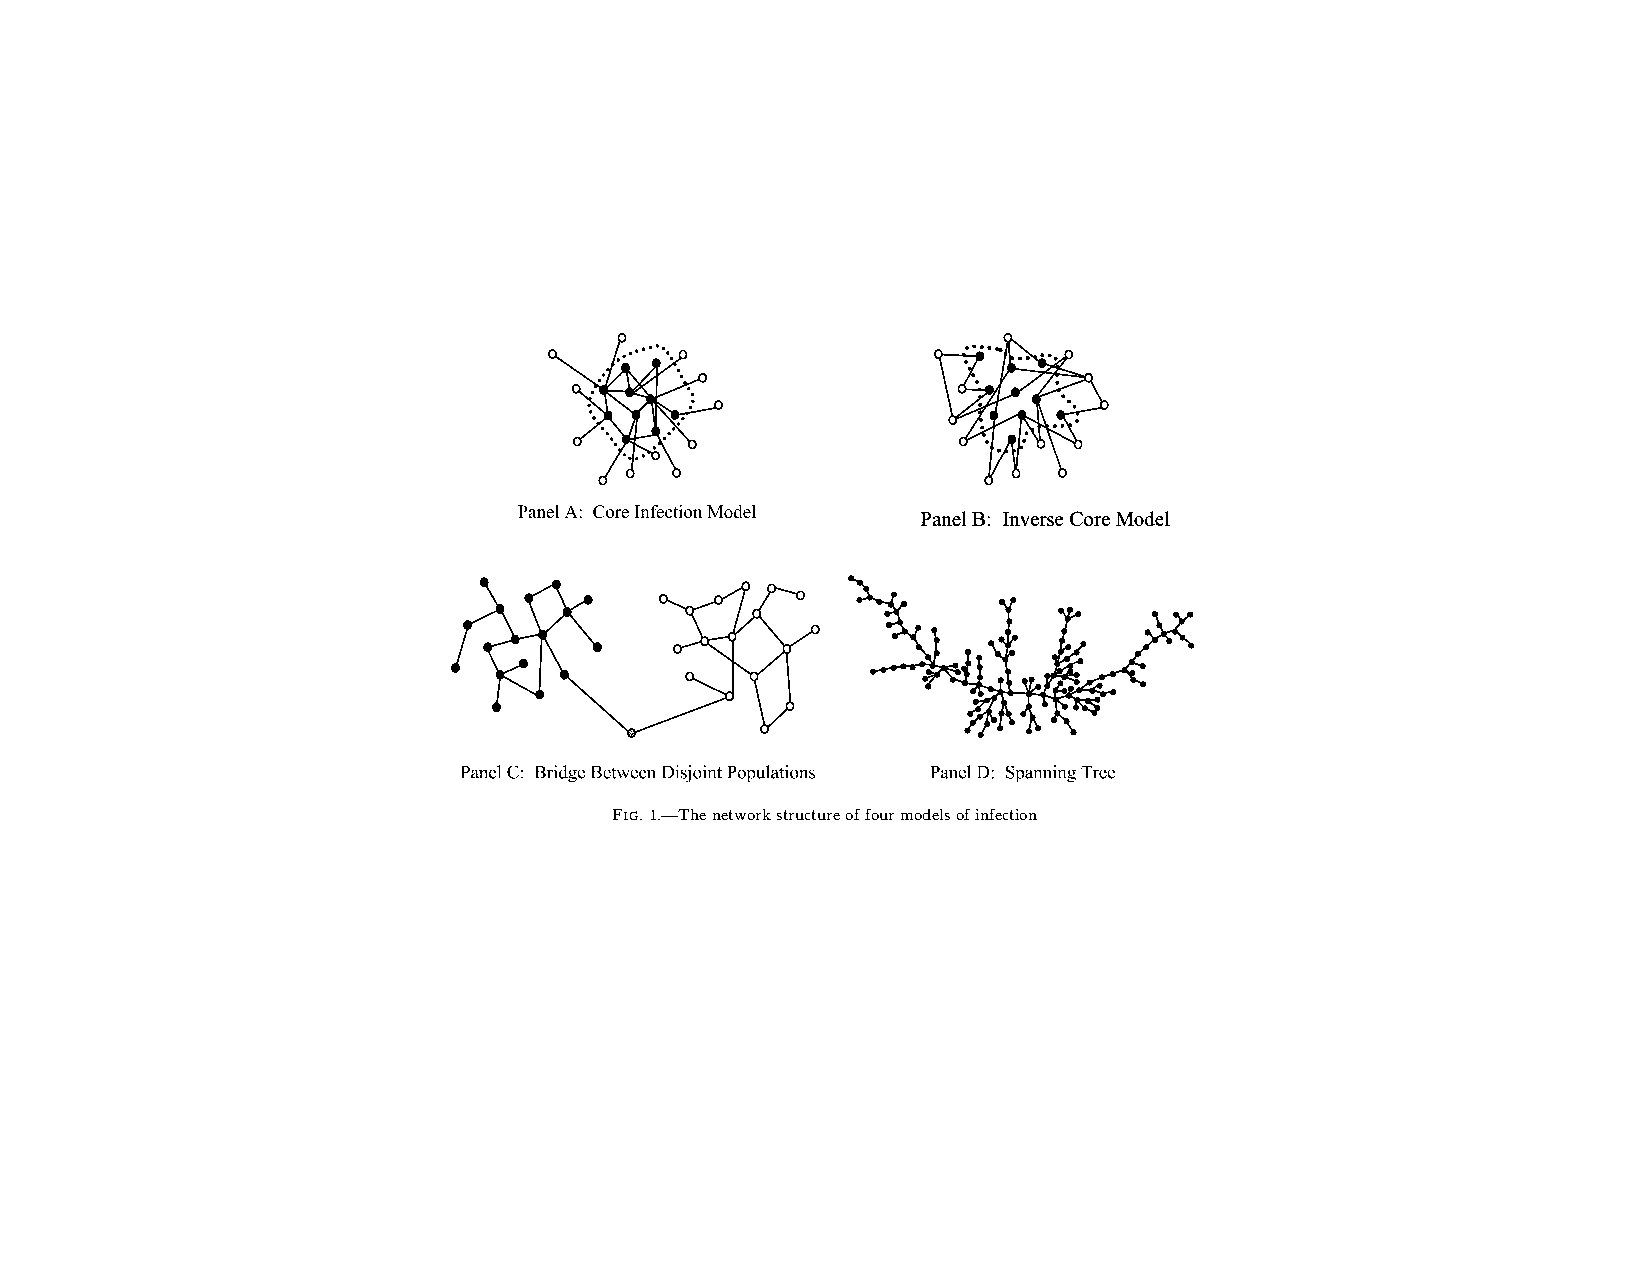
\includegraphics[width = 0.9\textwidth]{figures/bearman_chains_2004_fig1}
\end{center}

\note{
Random mixing might make sense for some diseases, but it seems like a bad model for STDs
What do real networks look like?


talk about each
bridge population is men who have sex with men and women
}

\end{frame}
%%%%%%%%%%%%%%%%%%%%%%%%%%%
\begin{frame}
\frametitle{}

\begin{center}
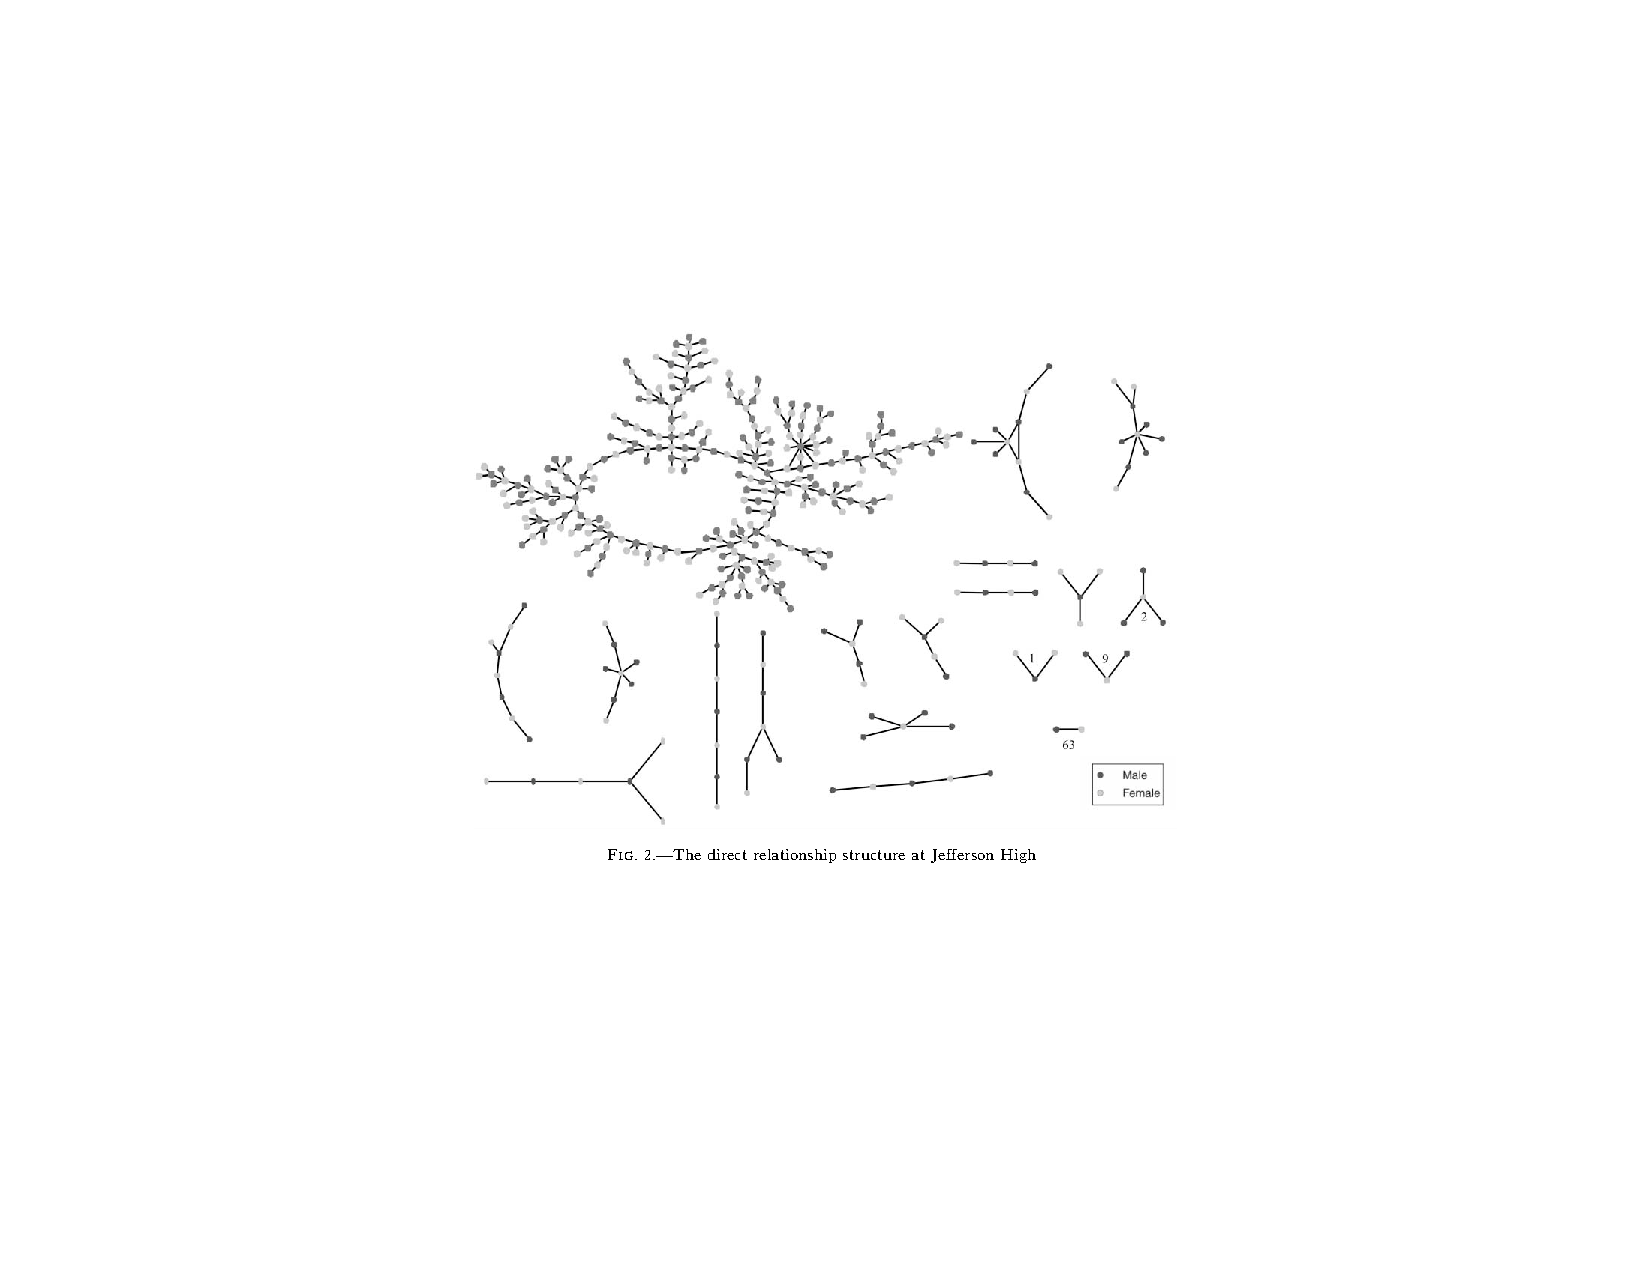
\includegraphics[width = 0.8\textwidth]{figures/bearman_chains_2004_fig2}
\end{center}

\note{

Jefferson High School represents an island population because it is relatively isolated.  Asked students three most recent special romantic relationships and three most recent sexual nonromantic relationship.  This yielded 447 partnerships.  

Jefferson High School had one giant component that was a spanning tree (figure~\ref{fig:bearman_chains_2004_fig2}).  This structure is very fragile.  

Also, note that STD risk is not just related to number of partners but how those partners fit into the larger structure.  Give Example of someone with two partners in the giant component and a sub-component.\\
}


\end{frame}
%%%%%%%%%%%%%%%%%%%%%%%%%%%
\begin{frame}
\frametitle{}

\setcounter{subfigure}{0}
\begin{figure}
  \centering
     \subfigure[Complete network data]{
     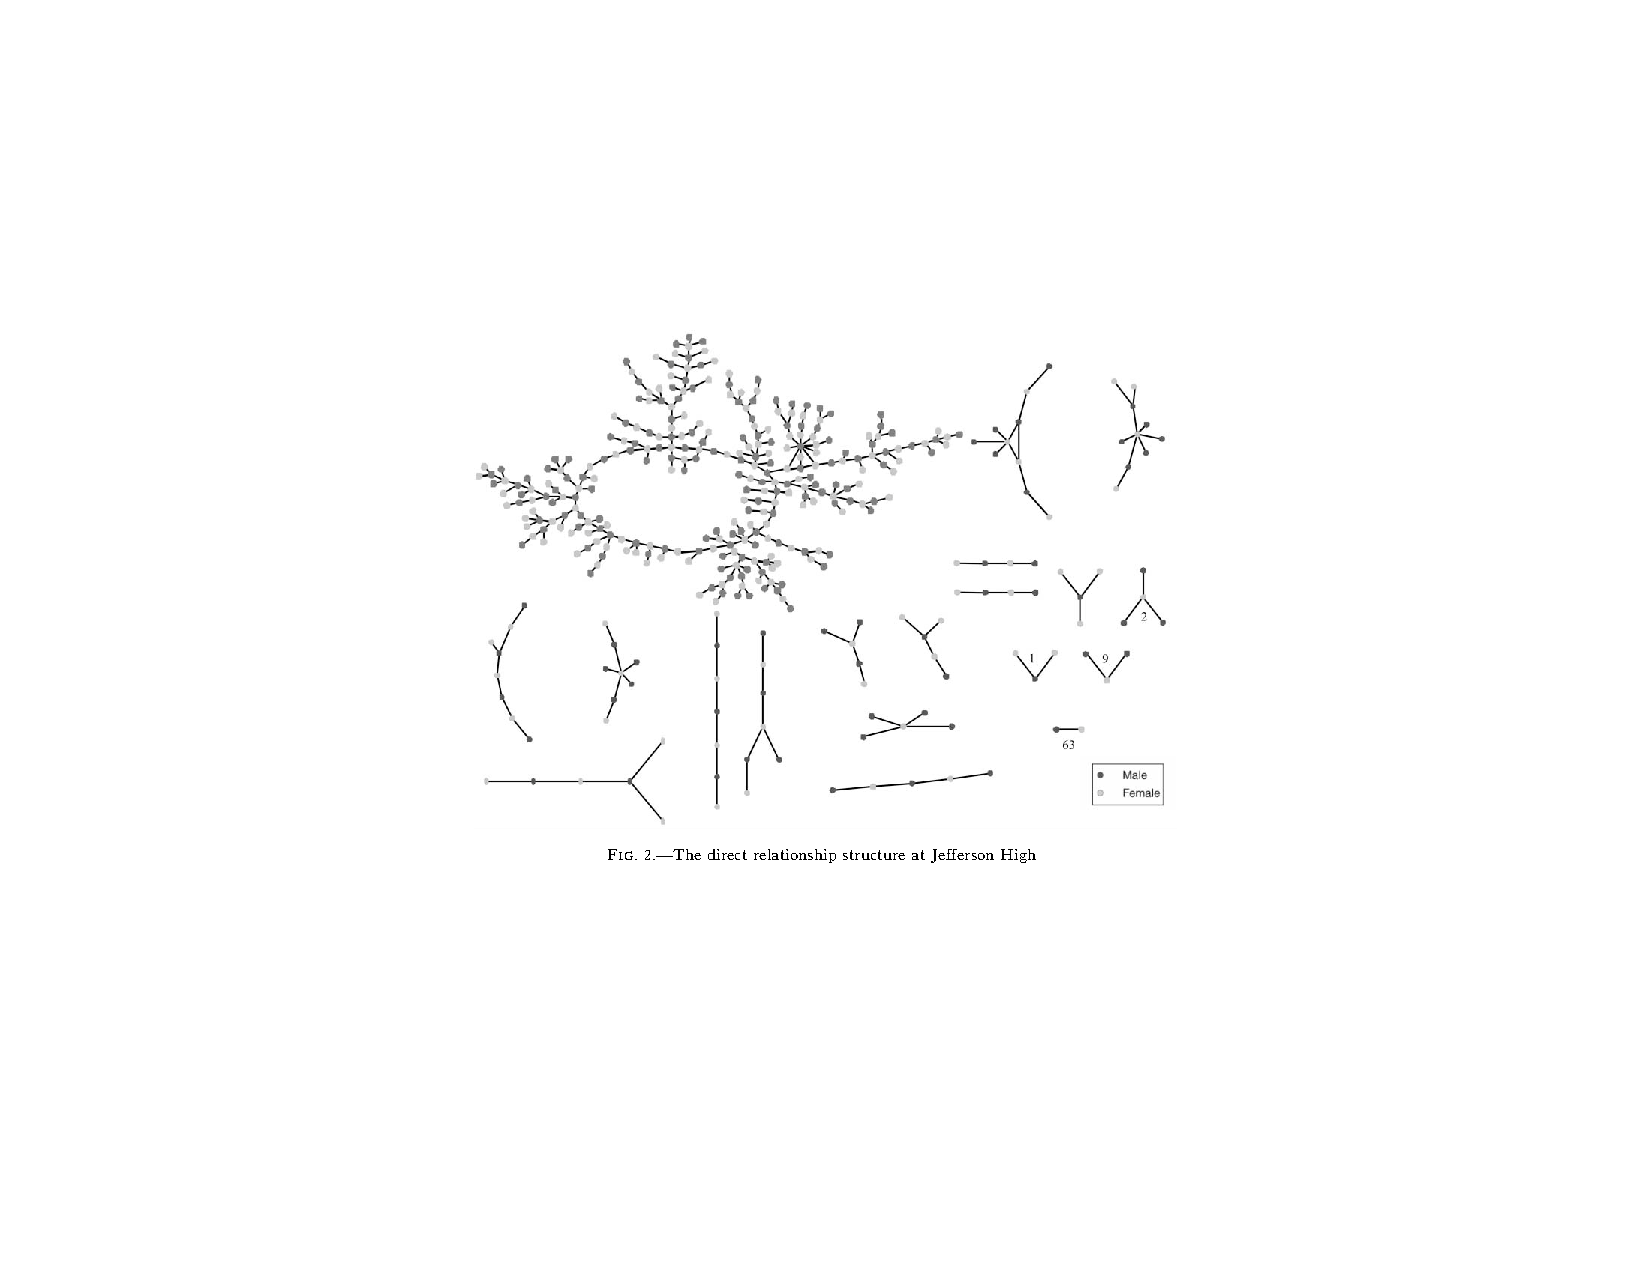
\includegraphics[width=0.45\textwidth]{figures/bearman_chains_2004_fig2}}
  \hspace{0in}
    \subfigure[Ego-centric network data]{
    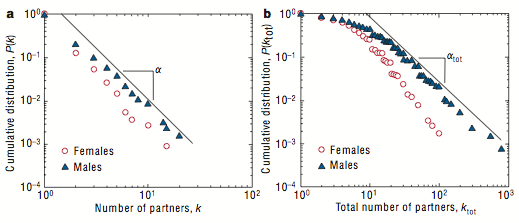
\includegraphics[width=0.45\textwidth]{figures/liljeros_web_2001_fig2}}
\end{figure}


\end{frame}
%%%%%%%%%%%%%%%%%%%%%%%%%%%%
\begin{frame}

What about time?

\setcounter{subfigure}{0}
\begin{figure}
  \centering
     \subfigure[Time flattened]{
     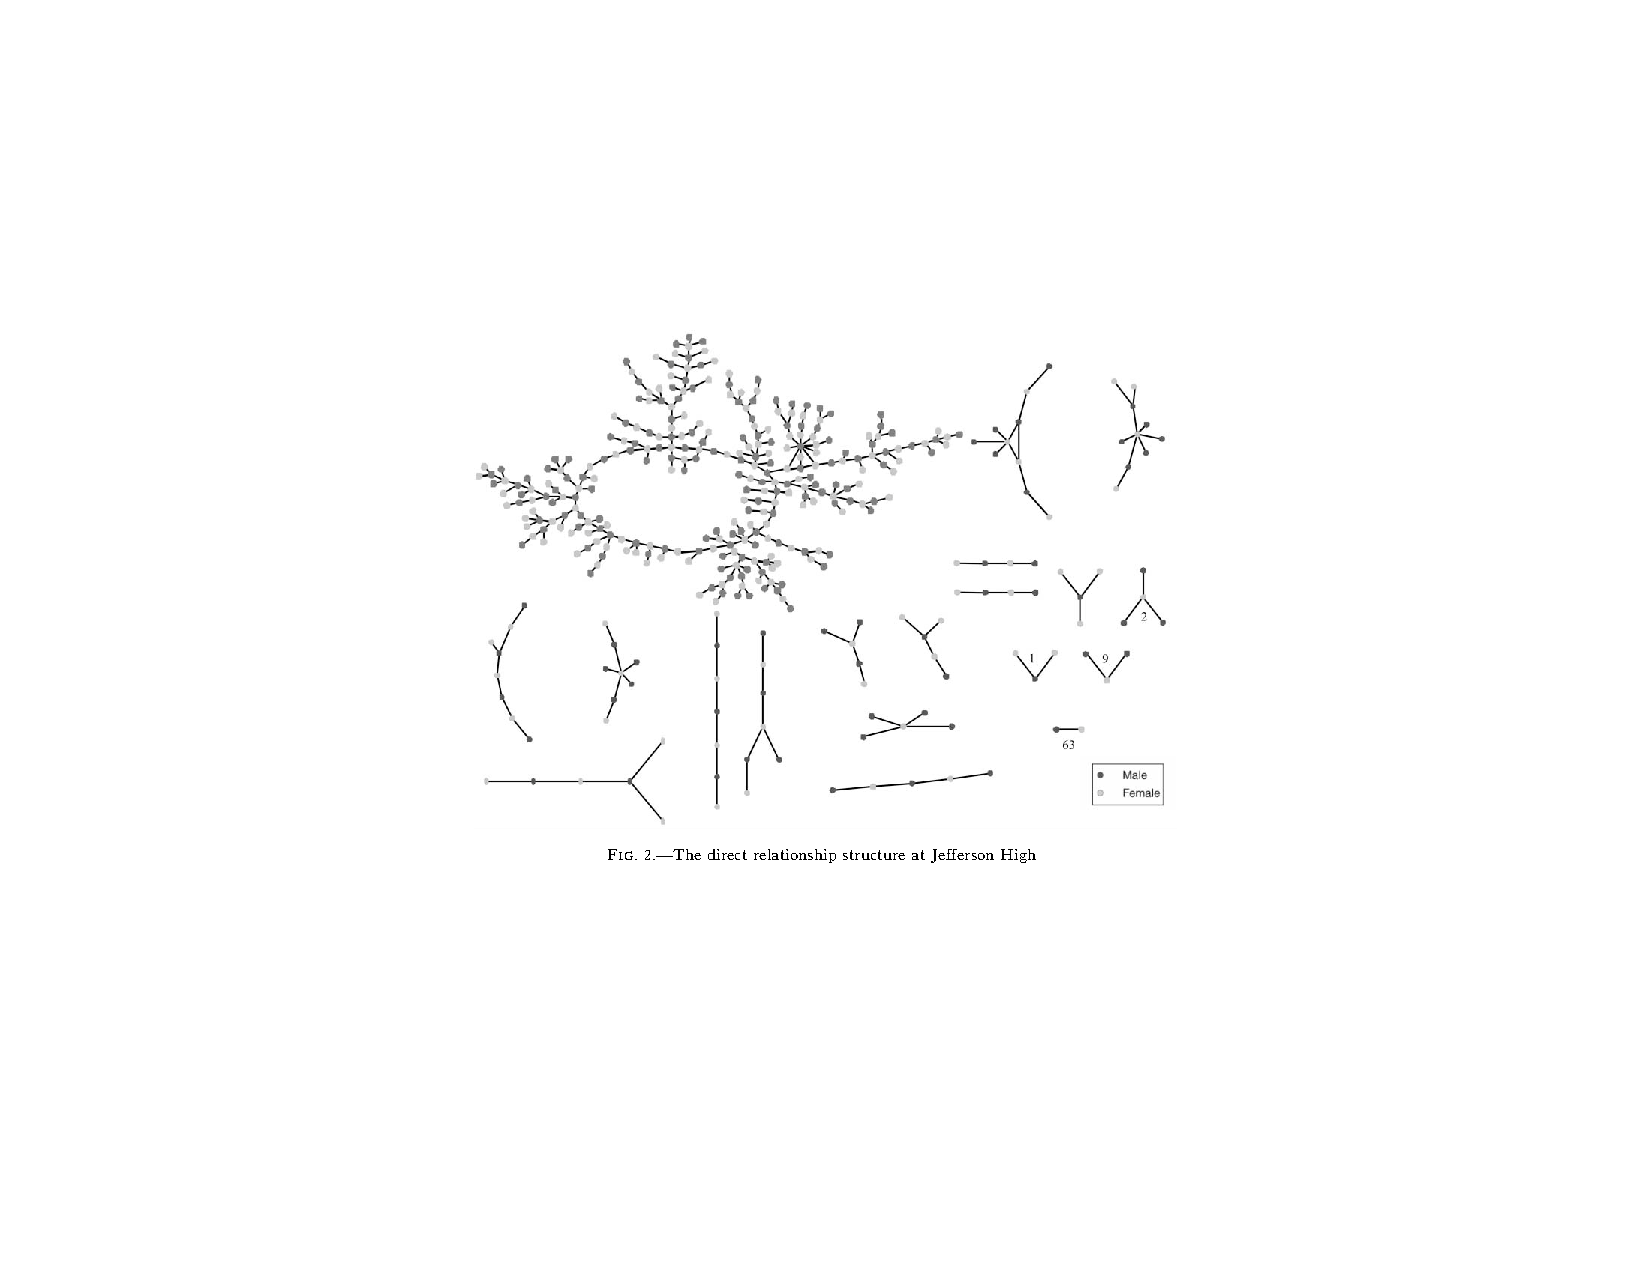
\includegraphics[width=0.45\textwidth]{figures/bearman_chains_2004_fig2}}
  \hspace{0in}
    \subfigure[Accounting for time]{
    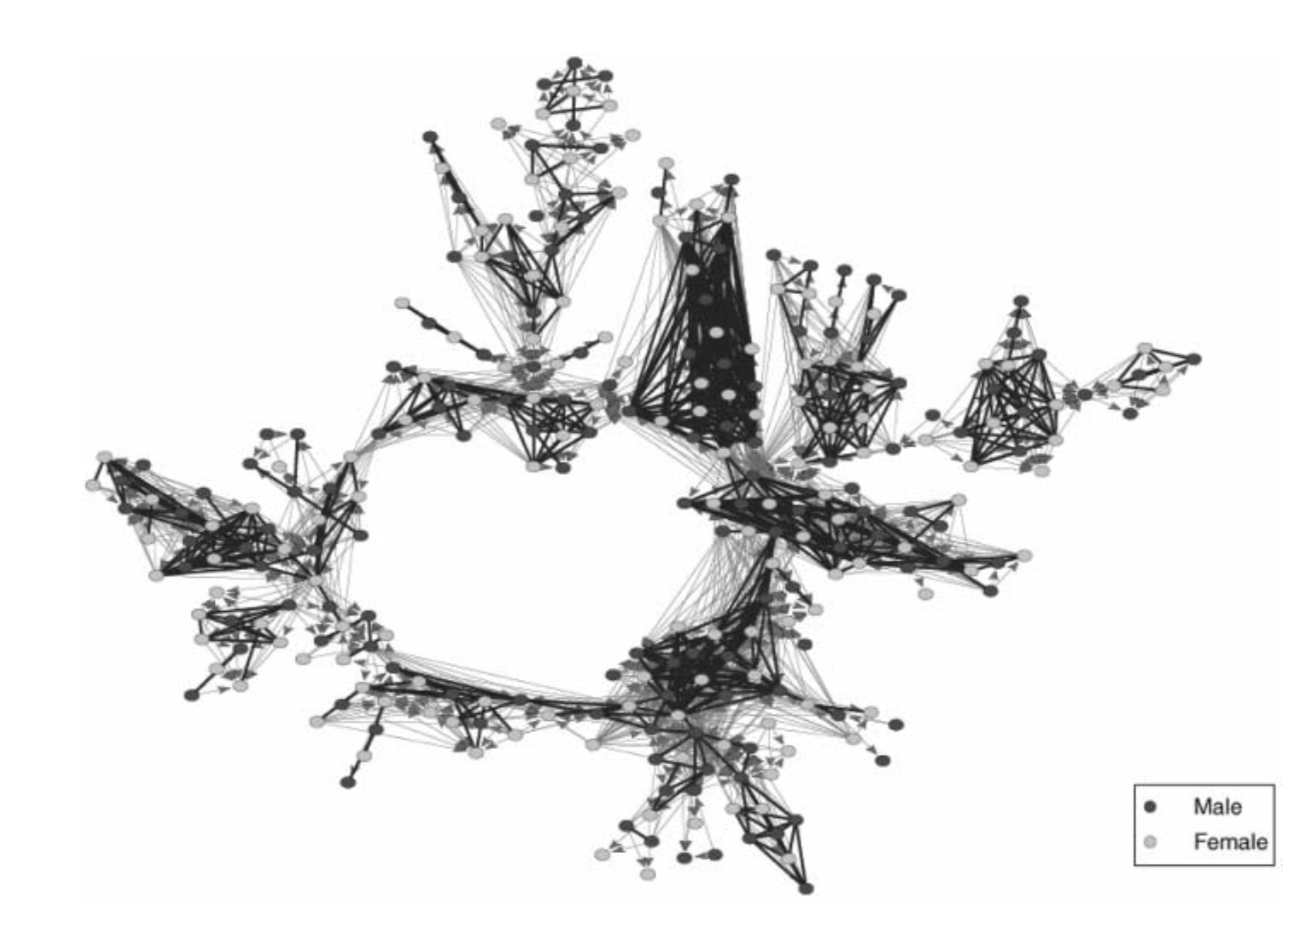
\includegraphics[width=0.45\textwidth]{figures/bearman_chains_2004_fig3}}
\end{figure}

\note{
Also note that time flattened picture \emph{overstates} the epidemic potential.  Now there is something a bit bogus about this because they compress time.  In reality those triads are not threesomes.  More generally, you can't catch an STD from your ex's future partners.  For example, before I met my lovely wife Amanda, I dated someone named Michele.  Image that after we broke-up she dated someone with gonorrhea and got it.  I can't then get it from her. 
}

\end{frame}
%%%%%%%%%%%%%%%%%%%%%%%%%%%
\begin{frame}

Generate 1,000 simulated networks with the same number of nodes and degree distribution, but where ties are formed completely randomly. How does these simulated networks compare to the observed network?
\pause
\begin{center}
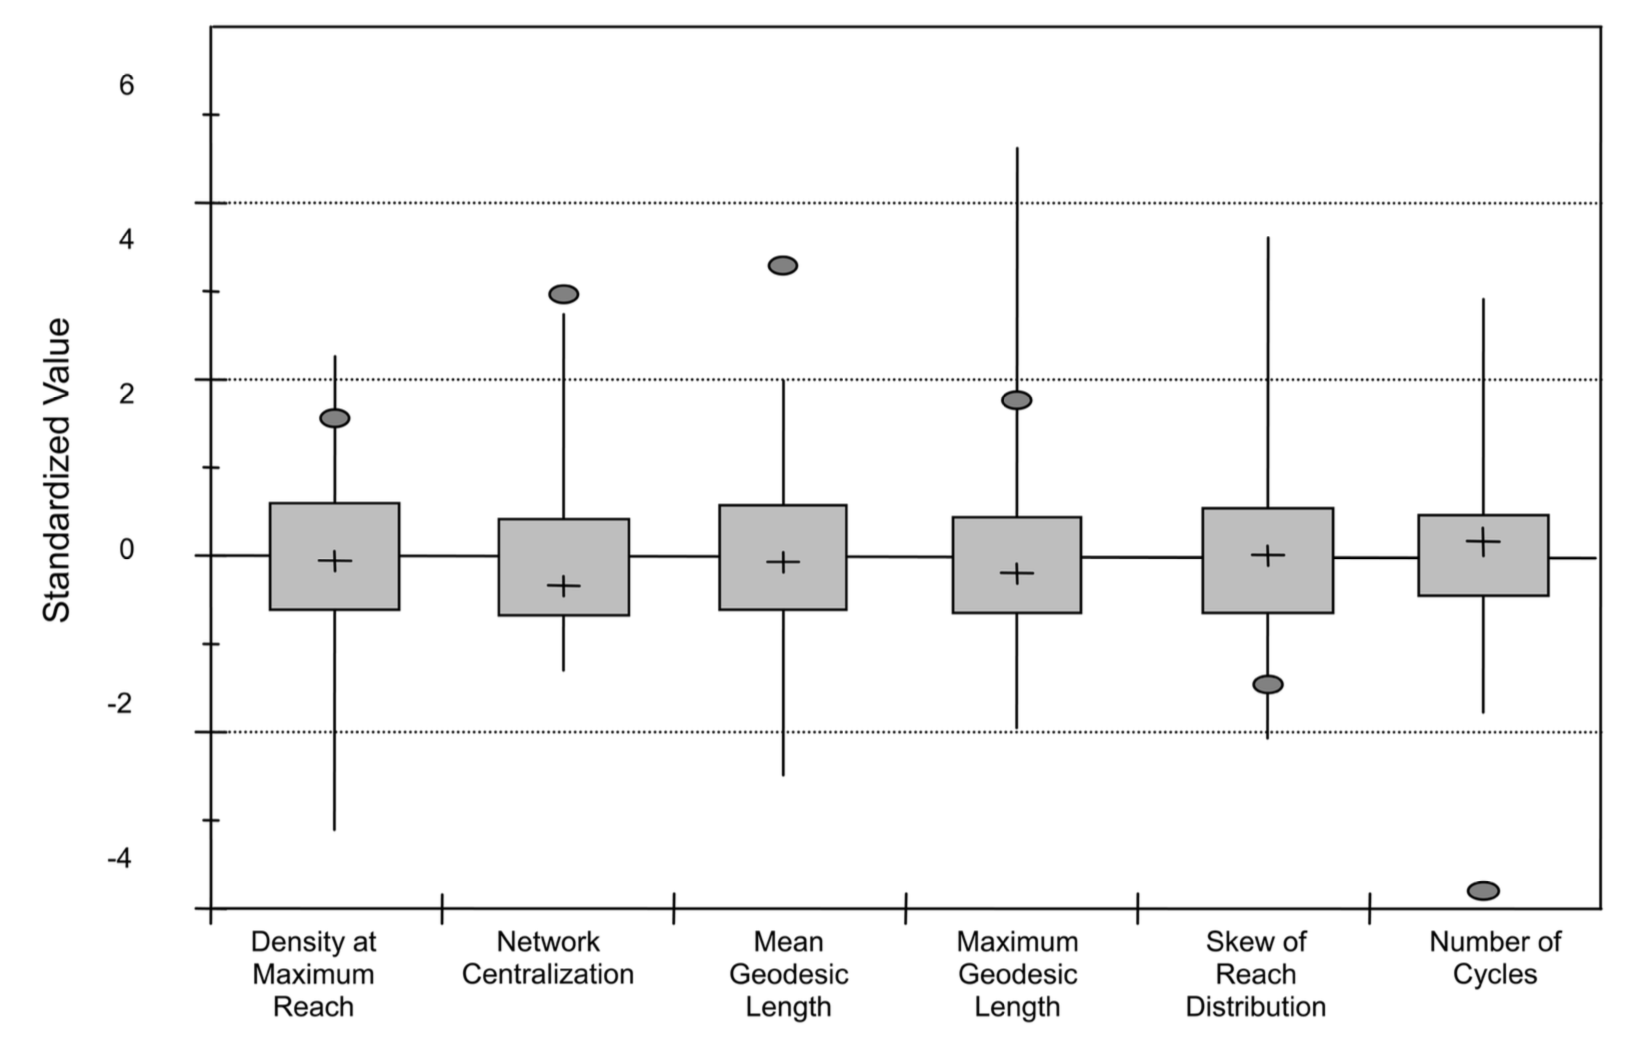
\includegraphics[width = 0.6\textwidth]{figures/bearman_chains_2004_fig6}
\end{center}

\note{
Simulated network are very different from observed networks.

This calls into question the rules that were used in the simulation
}

\end{frame}
%%%%%%%%%%%%%%%%%%%%%%%%%%
\begin{frame}

If this pattern did not arise randomly how did it come about?

\end{frame}
%%%%%%%%%%%%%%%%%%%%%%%%%%
\begin{frame}

\begin{center}
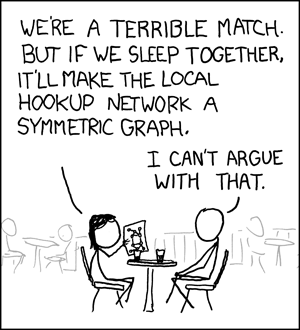
\includegraphics[height = 0.8\textheight]{figures/xkcd_convincing_pickup_line}
\end{center}

\vfill
\url{https://xkcd.com/403/}

\note{
probably not consciously created
}

\end{frame}
%%%%%%%%%%%%%%%%%%%%%%%%%%
\begin{frame}

\begin{center}
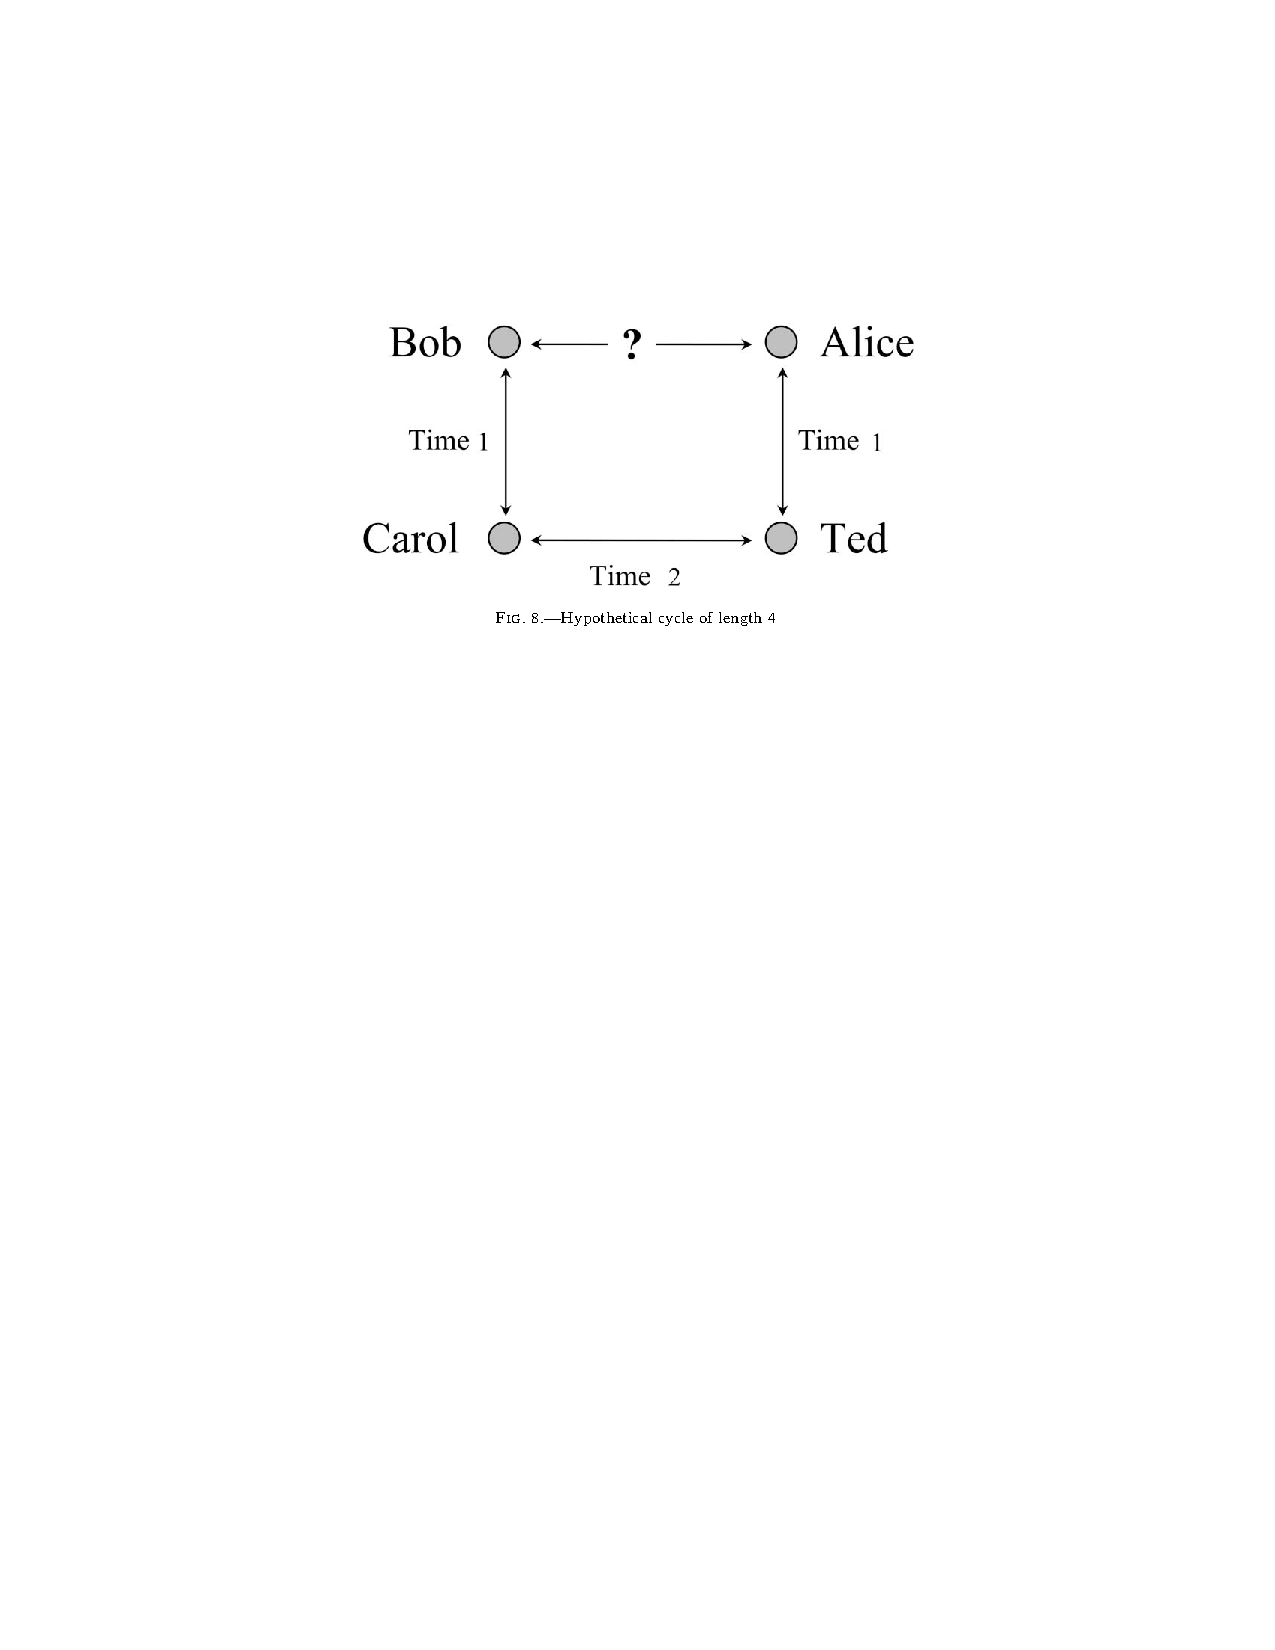
\includegraphics[width = 0.95\textwidth]{figures/bearman_chains_2004_fig8}
\end{center}

\note{
This simple rule explains why we should not see cycles of length 4
}

\end{frame}
%%%%%%%%%%%%%%%%%%%%%%%%%%%
\begin{frame}

\begin{center}
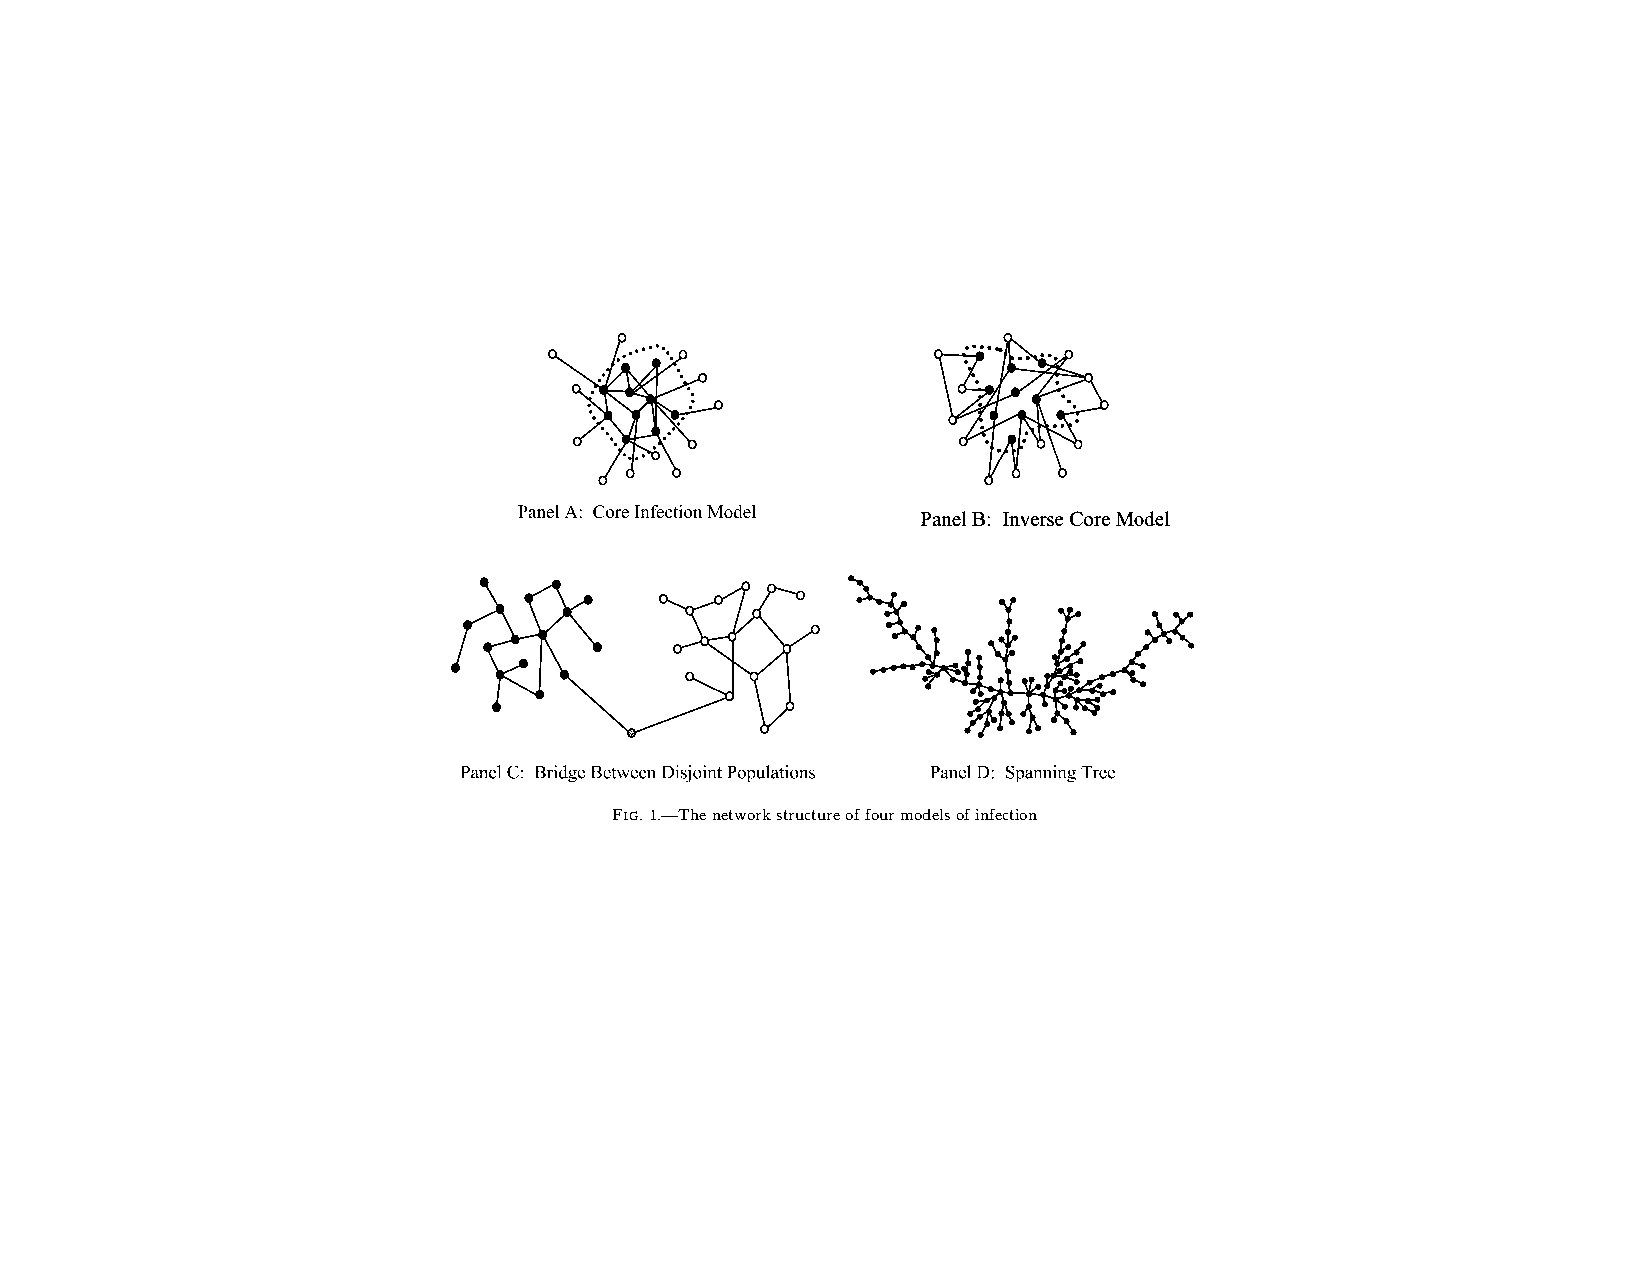
\includegraphics[width = 0.80\textwidth]{figures/bearman_chains_2004_fig1}
\end{center}

Policy implication: targeting might be important in a core network, but not as important in a spanning tree
\note{
This simple rule explains why we should not see cycles of length 4
}

\end{frame}
%%%%%%%%%%%%%%%%%%%%%%%%%%%%
\begin{frame}

Is this the same everywhere? In other words, what are the \emph{scope conditions} for this pattern?

\note{

\emph{Scope conditions}.  This is an important sociological concept.  Most things are not true everywhere (like gravity).  Scope conditions set out the boundaries of where we are likely to see this pattern.  Bearmen et al. think this is only true when actors can watch each other, might not occur in large cities.  However, we can only measure complete sexual networks in small isolated groups.  Thus, in all places where we might be able to measure sexual networks we might find this pattern.

}

\end{frame}
%%%%%%%%%%%%%%%%%%%%%%%%%%%
\begin{frame}

If we were able ethically and accurately measure the entire sexual network of Princeton students, do you think we would find a spanning tree?

\begin{enumerate}
\item yes
\item no
\end{enumerate}

\note{

If you said yes, that means this article convinced you of something.  that's cool.

}

\end{frame}

\end{document}
